\documentclass[12pt,a4paper]{article}
% math_setup.tex
% Essential Packages
\RequirePackage{etex}
\usepackage{comment}
\usepackage{etex}
\usepackage{listings}
\usepackage{amsmath}    % Advanced math typesetting
\usepackage{amsfonts}   % Math fonts
\usepackage{amssymb}    % Math symbols
\usepackage{amsthm}     % Theorem environment
\usepackage{mathtools}  % More symbols
\usepackage{tikz}       % For drawing diagrams
\usepackage{tikz-network}
\usepackage{pgfplots}
\usetikzlibrary{calc, arrows.meta, positioning, quotes}
\usepackage{mdframed}
\usepackage{float}
\usepackage{thmtools}
\usepackage{xcolor}
\usepackage{geometry}
\usepackage{fancyhdr}
\usepackage[colorlinks=true, linkcolor=blue, citecolor=green, urlcolor=red]{hyperref}
\usepackage{csquotes}
\usepackage[backend=biber, style=ieee]{biblatex}
\pgfplotsset{compat=1.18}
%\usepackage{mdframed}

% Wolfram Code Block
\lstdefinelanguage{Wolfram}{
    keywords={Sum, If, For, While, Do, Plot, Table, Range, Integrate, NIntegrate, D, Solve, NSolve, DSolve, NDSolve, LinearSolve, Expand, Factor, Simplify, FullSimplify, Module, Block, With},
    sensitive=true,
    morecomment=[l]{(*},
    morecomment=[s][\itshape]{(*}{*)},
    morestring=[b]",
    morestring=[b]',
}

\lstset{
    language=Wolfram,
    basicstyle=\ttfamily,
    keywordstyle=\color{blue}\bfseries,
    commentstyle=\color{green}\itshape,
    stringstyle=\color{red},
    showstringspaces=false,
    frame=single,
    breaklines=true,
    numbers=left,
    numberstyle=\tiny\color{gray},
    stepnumber=1,
    numbersep=5pt,
    backgroundcolor=\color{lightgray!20}
}

% add ref
\addbibresource{references.bib}
% Define colors
\definecolor{theoremcolor}{RGB}{230,230,250}  % Light purple
\definecolor{lemmacolor}{RGB}{240,248,255}    % Alice Blue
\definecolor{propcolor}{RGB}{240,255,240}     % Light green
\definecolor{corollarycolor}{RGB}{255,250,240} % Light orange
\definecolor{axiomcolor}{RGB}{255,240,245}    % Lavender blush
\definecolor{definitioncolor}{RGB}{240,255,255} % Light cyan
\definecolor{remarkcolor}{RGB}{245,245,245}   % Light gray
\definecolor{notationcolor}{RGB}{255,250,205}

% Boxed environments

\declaretheoremstyle[
    headfont=\normalfont\bfseries,
    bodyfont=\normalfont,
    headpunct={:},
    postheadspace=1em,
    mdframed={
        linecolor=black,
        backgroundcolor=definitioncolor,
        topline=true,
        bottomline=true,
        leftline=true,
        rightline=true,
        roundcorner=5pt
    }
]{boxeddefinitionstyle}

\declaretheorem[style=boxeddefinitionstyle, name=Definition]{definition}

\declaretheoremstyle[
    headfont=\normalfont\bfseries,
    bodyfont=\normalfont,
    headpunct={:},
    postheadspace=1em,
    mdframed={
        linecolor=black,
        backgroundcolor=theoremcolor,
        topline=true,
        bottomline=true,
        leftline=true,
        rightline=true,
        roundcorner=5pt
    }
]{boxedtheoremstyle}

% Theorem
\declaretheorem[style=boxedtheoremstyle, name=Theorem]{theorem}

% Lemma (adjust color)
\declaretheoremstyle[
    headfont=\normalfont\bfseries,
    bodyfont=\normalfont,
    headpunct={:},
    postheadspace=1em,
    mdframed={
        linecolor=black,
        backgroundcolor=lemmacolor,
        topline=true,
        bottomline=true,
        leftline=true,
        rightline=true,
        roundcorner=5pt
    }
]{boxedlemmastyle}
\declaretheorem[style=boxedlemmastyle, name=Lemma]{lemma}

% Proposition (adjust color)
\declaretheoremstyle[
    headfont=\normalfont\bfseries,
    bodyfont=\normalfont,
    headpunct={:},
    postheadspace=1em,
    mdframed={
        linecolor=black,
        backgroundcolor=propcolor,
        topline=true,
        bottomline=true,
        leftline=true,
        rightline=true,
        roundcorner=5pt
    }
]{boxedpropstyle}
\declaretheorem[style=boxedpropstyle, name=Proposition]{proposition}

% Corollary (adjust color)
\declaretheoremstyle[
    headfont=\normalfont\bfseries,
    bodyfont=\normalfont,
    headpunct={:},
    postheadspace=1em,
    mdframed={
        linecolor=black,
        backgroundcolor=corollarycolor,
        topline=true,
        bottomline=true,
        leftline=true,
        rightline=true,
        roundcorner=5pt
    }
]{boxedcorollarystyle}
\declaretheorem[style=boxedcorollarystyle, name=Corollary]{corollary}

% Axiom (boxed)
\declaretheoremstyle[
    headfont=\normalfont\bfseries,
    bodyfont=\normalfont,
    headpunct={:},
    postheadspace=1em,
    mdframed={
        linecolor=black,
        backgroundcolor=axiomcolor,
        topline=true,
        bottomline=true,
        leftline=true,
        rightline=true,
        roundcorner=5pt
    }
]{boxedaxiomstyle}
\declaretheorem[style=boxedaxiomstyle, name=Axiom]{axiom}

% Remark environment
\declaretheoremstyle[
    headfont=\normalfont\bfseries,
    bodyfont=\normalfont,
    headpunct={:},
    postheadspace=1em,
    mdframed={
        linecolor=black,
        backgroundcolor=remarkcolor,
        topline=true,
        bottomline=true,
        leftline=true,
        rightline=true,
        roundcorner=5pt
    }
]{remarkstyle}
\declaretheorem[style=remarkstyle, name=Remark, numbered=no]{remark}
% Normal, non-italic environments
\declaretheoremstyle[
    headfont=\normalfont\bfseries,
    bodyfont=\normalfont,
    headpunct={:},
    postheadspace=1em,
]{normalstyle}

% Notation environment
\declaretheoremstyle[
    headfont=\normalfont\bfseries,
    bodyfont=\normalfont,
    headpunct={:},
    postheadspace=1em,
    mdframed={
        linecolor=black,
        backgroundcolor=notationcolor,
        topline=true,
        bottomline=true,
        leftline=true,
        rightline=true,
        roundcorner=5pt
    }
]{boxednotationstyle}
\declaretheorem[style=boxednotationstyle, name=Notation]{notation}


% Note environment (more noticeable, with separators, no background, no end symbol)
\newenvironment{note}[1][]
    {\par\vspace{0.5em}\noindent\rule{\textwidth}{0.4pt}\par\vspace{0.5em}%
    \textbf{Note\if\relax\detokenize{#1}\relax\else: #1\fi}\par}
    {\par\vspace{0.5em}\noindent\rule{\textwidth}{0.4pt}\par\vspace{0.5em}}

\declaretheorem[style=normalstyle, name=Note, numbered=no]{oldnote}

\declaretheorem[style=normalstyle, name=Example]{example}
\declaretheorem[style=normalstyle, name=Exercise]{exercise}
\declaretheorem[style=normalstyle, name=Statement]{statement}
\declaretheorem[style=normalstyle, name=Solution, numbered=no]{solution}

% Proof environment (normal, non-italic, with QED symbol)
\declaretheoremstyle[
    headfont=\normalfont\bfseries,
    bodyfont=\normalfont,
    headpunct={:},
    postheadspace=1em,
    qed=$\blacksquare$
]{proofstyle}

\declaretheorem[style=proofstyle, name=Proof]{customproof}

% Shorthand
\newcommand{\vect}[1]{\mathbf{#1}} % For regular vectors
\newcommand{\uvec}[1]{\hat{\mathbf{#1}}} % For unit vectors
\newcommand{\prob}[1]{
    \section*{Problem #1}
}
\newcommand{\R}{\mathbb{R}} % Real numbers
\newcommand{\Z}{\mathbb{Z}} % Integers
\newcommand{\C}{\mathbb{C}} % Complex numbers
\newcommand{\N}{\mathbb{N}} % Natural numbers
\newcommand{\Q}{\mathbb{Q}} % Rational numbers
\newcommand{\Hq}{\mathbb{H}} % Quaternions
\newcommand{\F}{\mathbb{F}} % Finite fields
\newcommand{\Proj}{\mathbb{P}} % Projective space
\newcommand{\K}{\mathbb{K}} % Arbitrary field
\newcommand{\T}{\mathbb{T}} % Torus or sometimes denoted for Topological space
\newcommand{\A}{\mathbb{A}} % Affine space
\newcommand{\0}{\mathbf{0}} % Zero vector
\newcommand{\mbf}[1]{\mathbf{#1}} 
\newcommand{\mat}[1]{\mathbf{#1}}
\newcommand{\adj}{\operatorname{adj}}
\newcommand{\dom}[1]{
    \operatorname{dom}(#1)
}




% Layout
\geometry{a4paper, margin=1in}
\pagestyle{fancy}
\fancyhf{}
\rhead{\today}
\lhead{\textbf{ENG1005 Engineering Mathematics}}
\rfoot{Page \thepage}


\begin{document}
\title{ENG1005 Week2 Workshop Problem Set Solutions}
\author{Yang Xingyu (33533563)}
\date{\today}
\maketitle

\newcommand{\Ein}[1]{E^{\text{in}}(#1)}
\newcommand{\Eout}[1]{E^{\text{out}}(#1)}

\section*{Assumptions and notations}
\begin{remark}
What I have put in remark may not be directly related to the problem-solving, but just some of my mathematical ideas relate to the problem.

Also, as a Computer Science student from school of IT, I'd like to try using graph theory to solve these problems as a supplement.
\end{remark}
Before answering the problems in this problem set, we make the following assumptions and clarification of notations, which will be beneficial to analyze the problems.

We extend this road traffic model to an incomplete weighted simple directed graph, i.e., a graph that allow only one single directed edge between notes, and each edge has its own weight, which is the traffic flow measured in this scenario.
\begin{figure}[H]
    \centering
    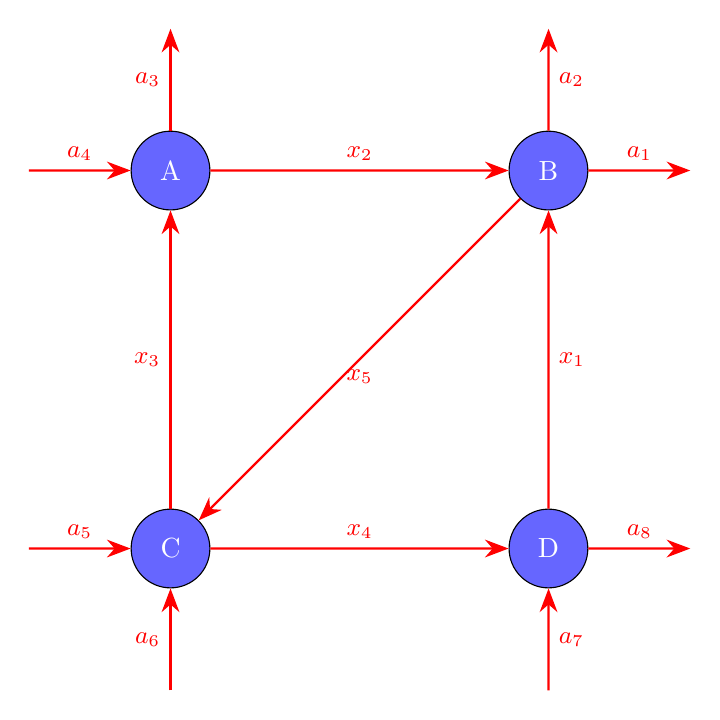
\begin{tikzpicture}[
    scale =1.2,
    node distance=4cm,
    main node/.style={circle, draw, fill=blue!60, text=white, minimum size=1cm},
    arrow/.style={-{Stealth[length=3mm]}, red, thick},
    label node/.style={font=\small}
]
% Main Nodes
\node[main node] (A) at (0,2) {A};
\node[main node] (B) at (4,2) {B};
\node[main node] (C) at (0,-2) {C};
\node[main node] (D) at (4,-2) {D};

% Horizontal arrows
\draw[arrow] (A) -- node[label node, above] {$x_2$} (B);
\draw[arrow] (C) -- node[label node, above] {$x_4$} (D);

% Vertical arrows
\draw[arrow] (C) -- node[label node, left] {$x_3$} (A);
\draw[arrow] (D) -- node[label node, right] {$x_1$} (B);

% Diagonal arrow
\draw[arrow] (B) -- node[label node, below] {$x_5$} (C);

% External arrows
\draw[arrow] ($(A)+(-1.5,0)$) -- node[label node, above] {$a_4$} (A);
\draw[arrow] ($(C)+(-1.5,0)$) -- node[label node, above] {$a_5$} (C);
\draw[arrow] (B) -- node[label node, above] {$a_1$} ($(B)+(1.5,0)$);
\draw[arrow] (D) -- node[label node, above] {$a_8$} ($(D)+(1.5,0)$);
\draw[arrow] (A) -- node[label node, left] {$a_3$} ($(A)+(0,1.5)$);
\draw[arrow] (B) -- node[label node, right] {$a_2$} ($(B)+(0,1.5)$);
\draw[arrow] ($(C)+(0,-1.5)$) -- node[label node, left] {$a_6$} (C);
\draw[arrow] ($(D)+(0,-1.5)$) -- node[label node, right] {$a_7$} (D);
\end{tikzpicture}
    \caption{Graph Representation of the Traffic}
    \label{fig:enter-label}
\end{figure}

We define the above graph $G = \{V,E\}$, where $V$ is the set of vertices and $E$ is the set of edges, and 
$$V=\{A,B,C,D\}, E=\{x_1,x_2,x_3,x_4,x_5,a_1,a_2,a_3,a_4,a_5,a_6,a_7,a_8\}.$$

Among which, $\{x_i\}_{i=1}^5$ are unknown internal flow of traffic, $\{a_i\}_{i=1}^8$ are known external flow (inwards or outwards) of traffic in the system.

\begin{notation}
We use notations $\deg(v)$, $W(e)$ to express the degree of $v$ and weight of $e$ respectively, where $v \in V,e\in E$.
\begin{remark}
    In this scenario, $W(e)$ represents the number of cars on the street in the given direction.
\end{remark}
\end{notation}

\begin{notation}
We use $E^{in}(v)$ and $E^{out}(v)$, where $v \in V$ to express the set of all edges that goes into, and out of vertex $v$, respectively. 
\begin{remark}
    In calculation, we may just use $x$ instead of $W(x)$ for simplicity.
\end{remark}
\end{notation}

\begin{notation}
We use $E_v$ to denote the set of edges that is connected to some vertex $v \in V$.
\end{notation}

Thus we have the following adjacency matrix (between known vertices):
\begin{equation}
\begin{bmatrix}
0 & x_2 & 0 & 0 \\
0 & 0 & x_5 & 0 \\
x_3 & 0 & 0 & x_4 \\
0 & x_1 & 0 & 0
\end{bmatrix},
\end{equation}
where each entry of the matrix is the weight of the corresponding edge.

\section*{Problem 1}
\begin{solution}
Since each of the nodes represents a crossing, then the inflow of cars equals the outflow of cars, as per the prerequisite provided by the problem set (all cars are keep moving and will not dissapear). We have the following relation for each of the node:
\begin{corollary}\label{in=out}
For any vertex $v$ in this graph $G$, the sum of the weight of all in-edges and sum of the weight of all out-edges must be equal, that is:
    $$\forall v \in V, \sum W(\Ein{v}) = \sum W(\Eout{v}).$$
\end{corollary}

By corollary \ref{in=out}, we have the following system of linear equations.
\begin{equation}\label{nodes_relations}
    \begin{cases}
x_{1} +x_{2} =a_{1} +a_{2} +x_{5} & ( Node\ B)\\
x_{5} +a_{5} +a_{6} =x_{3} +x_{4} & ( Node\ C)\\
x_{3} +a_{4} =a_{3} +x_{2} & ( Node\ A)\\
x_{4} +a_{7} =x_{1} +a_{8} & ( Node\ D)
\end{cases}
\end{equation}



\end{solution}
\section*{Problem 2}
\begin{solution}
Eight counters are not sufficient. This is because equation \ref{nodes_relations} is underdetermined. It is known that all $\displaystyle a_{x}$, $\displaystyle x\in \mathbb{Z}^{+\leqslant 8}$ are constants (measured by eight counters between internal streets and external streets). Even in the best case, where all equations are independent, four equations cannot get a specific solution for a 5-variable system of linear equations.

\begin{remark}
Another way to show this is using Rouché-Capelli theorem. But we need to get the reduced row echelon form for the system, which requires extra calculation. This is not what the question expect us to do.
    \begin{theorem}[Rouché-Capelli Theorem]\label{RCTheorem}
    Consider a system of linear equations $A\mathbf{x} = \mathbf{b}$, where $A$ is an $m \times n$ matrix, $\mathbf{x}$ is an $n \times 1$ vector of unknowns, and $\mathbf{b}$ is an $m \times 1$ vector. Let $[A|\mathbf{b}]$ denote the augmented matrix of the system. Then:
    
    \begin{enumerate}
        \item The system has at least one solution if and only if $\text{rank}(A) = \text{rank}([A|\mathbf{b}])$.
        \item If a solution exists, it is unique if and only if $\text{rank}(A) = n$.
    \end{enumerate}
    
    Therefore, the system has:
    \begin{itemize}
        \item No solution if $\text{rank}(A) < \text{rank}([A|\mathbf{b}])$
        \item Exactly one solution if $\text{rank}(A) = \text{rank}([A|\mathbf{b}]) = n$
        \item Infinitely many solutions if $\text{rank}(A) = \text{rank}([A|\mathbf{b}]) < n$
    \end{itemize}
\end{theorem}

In question 4, we got the REF of the system of linear equations, and it satisfies that $\text{rank}(A) = \text{rank}([A|\mathbf{b}]) < n$, and thus we have only general solutions, but not specific solution for the system.
\end{remark}



\end{solution}


\section*{Problem 3}
\begin{solution}
Only one more counter is needed, specifically to be used to count the number of cars travel on $\displaystyle x_{5}$.

Making $\displaystyle x_{5}$ a constant makes the previous system of linear equations solvable (has specific solution), since only node$\displaystyle \ B$ and node $\displaystyle C$ are involved by the flow on $\displaystyle x_{5}$, while the rest of the nodes are not affected by $\displaystyle x_{5}$. After setting the new counter, the system will become a system of four independent equations of four unknowns, which has specific solution.

\begin{remark}
While without further calculation, this makes sense, it is possible to further clarify. As we will show in later question, we actually need at least two new counter.

To show this in more details, we can split the variables and constants after assuming $x_5$ is some constant and combine all constant in each equation to some $c\in \Z$. This gives the following augmented matrix:
\begin{equation}
\left[
\begin{array}{cccc|c}
1 & 1 & 0 & 0 & c_1 \\
0 & 0 & 1 & 1 & c_2 \\
0 & -1 & 1 & 0 & c_3 \\
-1 & 0 & 0 & 1 & c_4
\end{array}
\right].
\end{equation}
For simplicity, we can check only the coefficient matrix, since we know we must have some constant in the last column of augmented matrix.

The coefficient matrix is 
\[
\begin{bmatrix}
1 & 1 & 0 & 0 \\
0 & 0 & 1 & 1 \\
0 & -1 & 1 & 0 \\
-1 & 0 & 0 & 1
\end{bmatrix}
\]
This can be reduced to
\[
\begin{bmatrix}
1 & 1 & 0 & 0 \\
0 & 1 & 0 & 1 \\
0 & 0 & 1 & 1 \\
0 & 0 & 0 & 0
\end{bmatrix}.
\]

By theorem \ref{RCTheorem}, the system of equation can either has general solution (infinitely many) or no solution, depending on what is in the last column of the augmented matrix (whether the last element is 0). If we assume that it is solvable, then we need to reduce the number of variable by one to get a specific solution, so we need two counters.
\end{remark}
\end{solution}

\section*{Problem 4}
\begin{solution}
Now we focus on equation \ref{nodes_relations} again. To write it in matrix form, we first separate the constants and variables. This gives us:
\begin{equation}\label{eqnodeafter}
    \begin{cases}
x_{1} +x_{2} -x_{5} =a_{1} +a_{2} & ( Node\ B)\\
x_{3} +x_{4}-x_5 =a_{5} +a_{6} & ( Node\ C)\\
x_{3} -x_{2} =a_{3} -a_{4} & ( Node\ A)\\
x_{4} -x_{1} =a_{8} -a_{7} & ( Node\ D)
\end{cases}.
\end{equation}

Now we can construct a $4\times 5$ coefficient matrix and $5\times 1$ variable matrix (a column vector of variables), whose product yields another $4\times 1$ column vector of constants.
\[
\begin{bmatrix}
1 & 1 & 0 & 0 & -1 \\
0 & 0 & 1 & 1 & -1 \\
0 & -1 & 1 & 0 & 0 \\
-1 & 0 & 0 & 1 & 0 
\end{bmatrix}
\begin{bmatrix}
x_1 \\
x_2 \\
x_3 \\
x_4 \\
x_5 
\end{bmatrix}
=
\begin{bmatrix}
a_1 + a_2 \\
a_5 + a_6 \\
a_3 - a_4 \\
a_8 - a_7 
\end{bmatrix}
\]

Substituting constants given, we have
\[
\begin{bmatrix}
1 & 1 & 0 & 0 & -1 \\
0 & 0 & 1 & 1 & -1 \\
0 & -1 & 1 & 0 & 0 \\
-1 & 0 & 0 & 1 & 0 
\end{bmatrix}
\begin{bmatrix}
x_1 \\
x_2 \\
x_3 \\
x_4 \\
x_5 
\end{bmatrix}
=
\begin{bmatrix}
45 \\
45\\
-10 \\
10
\end{bmatrix}.
\]

Convert to augmented form, we have
\[
\left[ \begin{array}{ccccc|c}
1 & 1 & 0 & 0 & -1 & 45 \\
0 & 0 & -1 & 1 & -1 & 45 \\
0 & -1 & 1 & 0 & 0 & -10 \\
-1 & 0 & 0 & 1 & 0 & 10 
\end{array} \right].
\]

Now we apply Gaussian Elimination algorithm.
\subsubsection*{Swap Row 4 with Row 1}
\[
\left[ \begin{array}{ccccc|c}
-1 & 0 & 0 & 1 & 0 & 10 \\
0 & 0 & -1 & 1 & -1 & 45 \\
0 & -1 & 1 & 0 & 0 & -10 \\
1 & 1 & 0 & 0 & -1 & 45 
\end{array} \right]
\]

\subsubsection*{Multiply Row 1 by -1}
\[
\left[ \begin{array}{ccccc|c}
1 & 0 & 0 & -1 & 0 & -10 \\
0 & 0 & -1 & 1 & -1 & 45 \\
0 & -1 & 1 & 0 & 0 & -10 \\
1 & 1 & 0 & 0 & -1 & 45 
\end{array} \right]
\]

\subsubsection*{Subtract Row 1 from Row 4}
\[
\left[ \begin{array}{ccccc|c}
1 & 0 & 0 & -1 & 0 & -10 \\
0 & 0 & -1 & 1 & -1 & 45 \\
0 & -1 & 1 & 0 & 0 & -10 \\
0 & 1 & 0 & 1 & -1 & 55 
\end{array} \right]
\]

\subsubsection*{Swap Row 4 with Row 2}
\[
\left[ \begin{array}{ccccc|c}
1 & 0 & 0 & -1 & 0 & -10 \\
0 & 1 & 0 & 1 & -1 & 55 \\
0 & -1 & 1 & 0 & 0 & -10 \\
0 & 0 & -1 & 1 & -1 & 45 
\end{array} \right]
\]

\subsubsection*{Add Row 2 to Row 3}
\[
\left[ \begin{array}{ccccc|c}
1 & 0 & 0 & -1 & 0 & -10 \\
0 & 1 & 0 & 1 & -1 & 55 \\
0 & 0 & 1 & 1 & -1 & 45 \\
0 & 0 & -1 & 1 & -1 & 45 
\end{array} \right]
\]

\subsubsection*{Add Row 3 to Row 4}
\[
\left[ \begin{array}{ccccc|c}
1 & 0 & 0 & -1 & 0 & -10 \\
0 & 1 & 0 & 1 & -1 & 55 \\
0 & 0 & 1 & 1 & -1 & 45 \\
0 & 0 & 0 & 2 & -2 & 90 
\end{array} \right]
\]

\subsubsection*{Row 3 times $\frac{1}{2}$}
\[
\left[ \begin{array}{ccccc|c}
1 & 0 & 0 & -1 & 0 & -10 \\
0 & 1 & 0 & 1 & -1 & 55 \\
0 & 0 & 1 & 1 & -1 & 45 \\
0 & 0 & 0 & 1 & -1 & 45
\end{array} \right]
\]
\begin{remark}
    We may stop here, since this matrix has already meet the requirements for RREF. We have
    \[
    \begin{cases}
        x_1-x_4=-10\\
        x_2+x_4-x_5=55\\
        x_3+x_4-x_5=45\\
        x_4-x_5=45
    \end{cases}
    \implies 
    \begin{cases}
        x_1-x_4=-10\\
        x_2 = 10\\
        x_3 = 0\\
        x_4 - x_5 = 45
    \end{cases}
    \]
    This means we need to introduce two parameter to get the solution. It can be confirmed that this solution is equivalent to the general solution we show later.
    \begin{note}
        This can be done earlier by further simplify the RREF by Row 2, row 3 minus row 4:
        \[
        \left[ \begin{array}{ccccc|c}
        1 & 0 & 0 & -1 & 0 & -10 \\
        0 & 1 & 0 & 0 & 0 & 10 \\
        0 & 0 & 1 & 0 & 0 & 0 \\
        0 & 0 & 0 & 1 & -1 & 45
        \end{array} \right].
        \]
    \end{note}

    But for consistency, we will rearrange it to the way we did in the lecture slides.
\end{remark}
We can let row 4 subtracted by it self to get a row of zero vector, since every row can yields a o zero vector by minus itself. This does not affect the fact that the augmented matrix is still RREF, since RREF allows a row of full zero entries to be at the bottom.
\begin{note}
This is also a very visually approachable way to show that a system has only general solution, i.e., a solution that need to be parameterized. Because zero vector does not provide any information, or rather, constraints, in this case of system of equations.
\end{note}


Finally, by letting the last row subtracted by itself, we have the RREF:
\begin{equation}\label{RREF}
\left[ \begin{array}{ccccc|c}
1 & 0 & 0 & -1 & 0 & -10 \\
0 & 1 & 0 & 1 & -1 & 55 \\
0 & 0 & 1 & 1 & -1 & 45 \\
0 & 0 & 0 & 0 & 0 & 0 
\end{array} \right].
\end{equation}
\end{solution}

\section*{Problem 5}
\begin{solution}
From the RREF we obtained in (\ref{RREF}), we can deduce that we need two parameter to describe (one of) the general solution. We have five variables but three independent equations can only assure three certain variable. Full zero in the last row implies one variable must be free variable, and the non-existent fifth equation that is required for the existence of a specific solution implies we have the other free variable. Thus, we need to introduce two parameter.

We introduce two free variables \( x_4= s \) and \( x_5=t \), and get the following solution (not unique):
\[
\begin{cases}
x_1 = s - 10 \\
x_2 = -s + t + 55 \\
x_3 = -s + t + 45 \\
x_4 = s \\
x_5 = t
\end{cases}
\]
where \( s \) and \( t \) are free parameters.

We can write this as a linear combination of vectors.
\[
\begin{bmatrix}
x_1 \\
x_2 \\
x_3 \\
x_4 \\
x_5
\end{bmatrix}
=
\begin{bmatrix}
-10 \\
55 \\
45 \\
0 \\
0
\end{bmatrix}
+
s \begin{bmatrix}
1 \\
-1 \\
-1 \\
1 \\
0
\end{bmatrix}
+
t \begin{bmatrix}
0 \\
1 \\
1 \\
0 \\
1
\end{bmatrix}
\]
\begin{remark}
This solution actually has some very interesting meaning. 
\begin{itemize}
    \item We know that, the solution $s = (x_1, x_2, x_3, x_4, x_5)$ satisfies $s \in \R^5$, and the set of all possible solution $S$ satisfies $S \subset \R^5$. This is because the set all solutions is a subspace of $\R^5$.
    \item From the perspective of function and mapping, the solution actually defines a mapping $f:\F^2 \to \F^5$ defined by 
    $$f(s,t) := \begin{bmatrix}
-10 \\
55 \\
45 \\
0 \\
0
\end{bmatrix}
+
s \begin{bmatrix}
1 \\
-1 \\
-1 \\
1 \\
0
\end{bmatrix}
+
t \begin{bmatrix}
0 \\
1 \\
1 \\
0 \\
1
\end{bmatrix}.$$

Where $\F$ is some number filed depends on how we define, or choose the parameter $s$ and $t$ ($\Z$ in this scenario).

This can be analogised to: using 
$\begin{bmatrix}
-10 \\
55 \\
45 \\
0 \\
0
\end{bmatrix}$
as origin,  
$\begin{bmatrix}
1 \\
-1 \\
-1 \\
1 \\
0
\end{bmatrix}$
and 
$\begin{bmatrix}
0 \\
1 \\
1 \\
0 \\
1
\end{bmatrix}$
as base vector, creating a new coordinate in $\F^5$, and thus we could get something similar to a plane, which is why we call the solution set "hyperplane", and the parameters $s,t$ define how we compound new coordinate using these elements in $\R^5$. 

\item It can also be noticed that, when the number of parameters in the solution changes, the subspace changes accordingly. We let $n$ be number of unknown variables in a \textbf{solvable} linear system, and $p$ be the number of parameter required to represent the solution. When $p = 0$, the solution set is $\F^0$, which is basically a point. When $p = n$, it's a completely opposite case, the set of solution is still $\F^n$, where you can manipulate everything. 

Thinking inductively, we may show that for all solvable linear systems, the set of solution is decided by the number of parameters required to represent a solution. For any $0 \leq p \leq n$, the set of all solution for the system will be some subspace $\F^p$ of $\F^n$. Thus, when we have one parameter, the solutions will be a line in that space, if two, a plane, if three, it will be something solid, etc.
\item After conducting further research, I find that this solution set is commonly referred to as an affine subspace. 
\begin{definition}[Affine Subspace]
An affine subspace of a vector space \( \mathbb{F}^n \) is a subset of the form
\[
\mathbf{p} + L = \{ \mathbf{p} + \mathbf{v} \mid \mathbf{v} \in L \}
\]
where \( \mathbf{p} \) is a fixed point in \( \mathbb{F}^n \) and \( L \) is a linear subspace of \( \mathbb{F}^n \). If \( L \) is a \( k \)-dimensional subspace, then the affine subspace \( \mathbf{p} + L \) is called a \( k \)-dimensional affine subspace.
\end{definition}
The \( \mathbf{p} \) here is exactly the constant vector in the solution, and \( L \) is the sum of all vectors with parameterised scalar, which is obviously a subspace of \( \mathbb{F}^n \).
\end{itemize}

\end{remark}
\end{solution}

\section*{Problem 6}
\begin{solution}
After further clarified by the general solution we obtained from RREF, we can confirm that we need another two counters. This is because to make sure the system of linear equations is stable (has specific solution), we must make sure we know at least two parameters. In our case, we need to set one counter on edge $x_4$ and the other one on $x_5$.

To further illustrate, we will prove that the system will have specific solution after we add the two counters.
\begin{proof}
    Assume that $x_4, x_5$ are measured as $c_1,c_2$ respectively by the counters.
    
    Then, by substituting $x_4 = c_1$, $x_5=c_2$ to (\ref{eqnodeafter}) and rearrange, the system will be:
    \[
    \begin{cases}
        x_1+x_2 = 45+c_1\\
        x_3 = 45-c_1+c_2 \\
        x_3-x_2 = -10\\
        x_1=c_1-10
    \end{cases}
    \]
    This system is obviously overdetermined, since all four equations are independent. and we have more equations (four) than we need to find specific solutions for three unknowns ($\{x_i\}_{i=1}^3$).
\end{proof}
Thus, we have shown that adding two counters allows us to find a specific solution.
\end{solution}
\section*{Problem 7}
\begin{solution}
The solution 
\[
\begin{bmatrix}
x_1 \\
x_2 \\
x_3 \\
x_4 \\
x_5
\end{bmatrix}
=
\begin{bmatrix}
-10 \\
55 \\
45 \\
0 \\
0
\end{bmatrix}
+
s \begin{bmatrix}
1 \\
-1 \\
-1 \\
1 \\
0
\end{bmatrix}
+
t \begin{bmatrix}
0 \\
1 \\
1 \\
0 \\
1
\end{bmatrix}
\]
can be interpreted as follows.
\begin{itemize}
    \item The constant part, $[-10,55, 45,0,0]^T$ can be interpreted as the initial status of the system. Though some are negative, it does not really matter here, since we only need to make sure that all components in the solution are greater than zero. 
    \item For the parameter $s$ and $t$, we must have $(s,t)\in \N_0 \times \N_0$, because we must make sure the solution is a non-negative integer.
    \item The vector accompanied by $s$, $[1,-1,-1,1,0]^T$ can be known as, whenever $s$ is increased by one, the number of cars in $x_1,x_4$ will increase by one while decrease one in $x_2,x_3$. That is, the number of cars leaving edges $x_2,x_3$, will flow into $x_1,x_4$ (In the internal system).
 \begin{remark}
        Let the internal graph $G_{in} = (V, E_{in})$ where $E_{in} = \{x_1, x_2, x_3, x_4, x_5\}$, and define the subgraph $T = \{x_3, x_2, x_5, x_4, x_1\}$ as an ordered set. This graph is the only Eulerian path in $G_{in}$. In this path, assuming the vehicle starts at $C$, it can only move through $x_3$ to reach $A$. Then, it can only move along $x_2$ to reach $B$, then through $x_5$ back to $C$, and finally through $x_4$ and $x_1$ back to $B$. In this closed system, the cars moving along $x_2$ or $x_3$ must reach $x_1$ and $x_4$, so $s$ is essentially a "scalar" that determines the number of such cars in the system.
        
        This can also explain why $x_5$ is a tricky part (free variable) of the system. When the vehicle reaches the destination $B$, the only available route is $x_5$. This explains why $x_5$ must be measured to stabilise the system because the traffic flow on $x_5$ is dependent on the system itself. This is similar to a recursive relationship, derived through basic algebraic operations, and has different but equivalent way to represent algebraically.
    
    \end{remark}
    \item For the last part, the vector $[0,1,1,0,1]^T$ scaled by parameter $t$, shows that the cars running on $x_2,x_3,x_5$ must has equal increase or decrease, and parameter $t$ can be interpreted as the number of cars running on (or leaving) this section of the internal street.
  \begin{remark}
        Similarly, we can use graph theory to explain this part. This part of the graph is also a cycle. Therefore, when we separate the inner streets from the external system, the cars cycle within the same path repeatedly and cannot leave the cycle, meaning that the number of cars in this part will increase or decrease simultaneously.
        \begin{note}
            While the symmetric subgraph of this cycle does not appear as a parameterized term in the solution, the information is already implied in the last vector discussed. Therefore, these two scaled vectors contain all the information required to construct the system of linear equations modeling graph $G$. If this is true, then the first constant vector can be interpreted as the external factor influencing the system in this scenario.

            Thus, by analyzing this linear system, we reach a surprisingly concise but profound conclusion: \textbf{This system of linear equations represents the new state of the graph given these known external and internal factors.}

            These two scaled vectors perfectly simulate the rules or logic of the traffic system, and we achieved all this through basic algebraic operations, which is quite amazing!
        \end{note}
    \end{remark}
\end{itemize}
\end{solution}
\section*{Problem 8}
\begin{solution}
Now we apply some implied constraints on the solution to further narrow down our solution space. As all $x_i \in \{x_i\}_{i=1}^5$ represents the average numbers of cars per hours in the corresponding part in the internal streets, so $x_4>0$. To make sure this is true, we can pick and rearrange the part in the solution that involves $x_4$ and build a new system of linear inequality.
\[
\begin{cases}
x_1 = s - 10 \\
x_2 = -s + t + 55 \\
x_3 = -s + t + 45 \\
x_4 = s
\end{cases}
\implies
\begin{aligned}
    &x_4 = 10 +x_1 \geq 0 && (1)\\
    &x_4 = t+55-x_2 \geq 0 && (2)\\
    &x_4 = t + 45 -x_3 \geq 0 && (3)\\
    &x_4 \geq 0 && (4)
\end{aligned}
\]

Since $\forall x\in \{x_i\}_{i=1}^5, x \geq 0$, (1) is enough to show that $x_4 \geq 10$, i.e., $\min(x_4)=10$. So, mathematically, at least 10 cars will be counted in $x_4$ per hour on average.

\end{solution}
\section*{Problem 9}
To get the minimum of the full inner system, we can just sum up all the components in the solution.
\begin{solution}
\[
\begin{cases}
x_1 = s - 10 \\
x_2 = -s + t + 55 \\
x_3 = -s + t + 45 \\
x_4 = s \\
x_5 = t
\end{cases}
\implies 
\sum_{i=1}^5 x_i = 3t -10 + 55 + 45 = 3t + 90 
\]

So we have $\sum_{i=1}^5 x_i \geq 90$, since $t \geq 0$.

To figure out the exact flow of cars in the system when the sum of internal car flow is minimised, we may consider discover the minimum number of cars in each section of the internal streets, since 
$$\min(\sum_{i=1}^5 x_i) = \sum_{i=1}^5\min(x_i)$$
is always true given that $\forall x\in \{x_i\}_{i=1}^5, x_i \geq 0$.

From the previous problem, we have $x_4 \geq 10$, and we also have $x_5\geq 0$. 
\begin{itemize}
    \item As $x_4 \geq 10$,  $x_4 - 10 \geq 0$ and thus $x_1 \geq 0$.
    \item $x_5 \geq 0 \implies x_3 \geq 35 $.
    \item $x_2 \geq 45$ by we obtained previously.

\end{itemize}
To sum up,
\begin{equation}
    \begin{cases}
        x_1 = x_4 -10 \geq 0\\
        x_2 \geq -10 + 0 + 55\\
        x_3 = -10 + t + 45 \geq 0\\
        x_4 \geq 10\\
        x_5 = t \geq 0
    \end{cases}
    \implies
    \begin{cases}
        x_1 \geq 0\\
        x_2 \geq 45\\
        x_3 \geq 35\\
        x_4 \geq 10\\
        x_5 \geq 0
    \end{cases}.
\end{equation}

Now, we can draw the traffic flow when the minimum number of cars is achieved.

\begin{figure}[H]
    \centering
    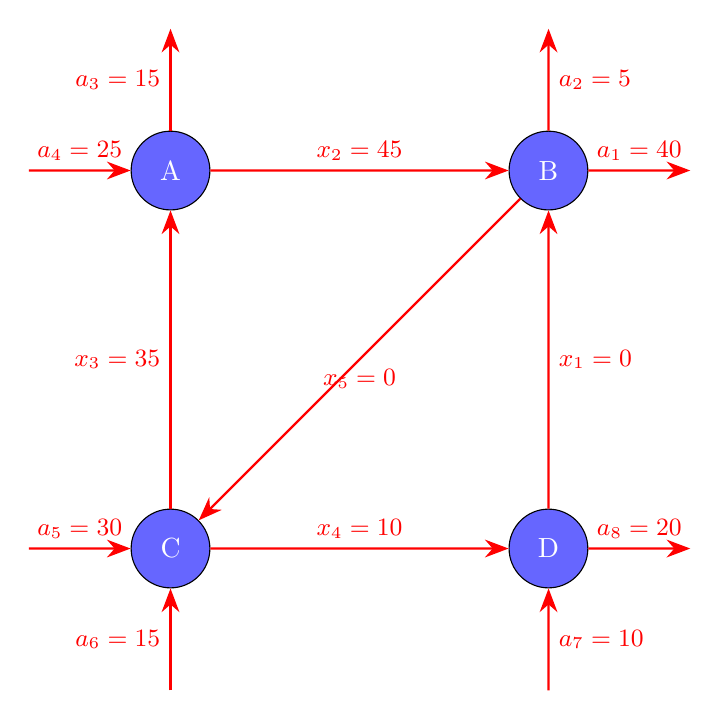
\begin{tikzpicture}[
    scale =1.2,
    node distance=4cm,
    main node/.style={circle, draw, fill=blue!60, text=white, minimum size=1cm},
    arrow/.style={-{Stealth[length=3mm]}, red, thick},
    label node/.style={font=\small}
]
% Main Nodes
\node[main node] (A) at (0,2) {A};
\node[main node] (B) at (4,2) {B};
\node[main node] (C) at (0,-2) {C};
\node[main node] (D) at (4,-2) {D};

% Horizontal arrows
\draw[arrow] (A) -- node[label node, above] {$x_2=45$} (B);
\draw[arrow] (C) -- node[label node, above] {$x_4=10$} (D);

% Vertical arrows
\draw[arrow] (C) -- node[label node, left] {$x_3=35$} (A);
\draw[arrow] (D) -- node[label node, right] {$x_1=0$} (B);

% Diagonal arrow
\draw[arrow] (B) -- node[label node, below] {$x_5=0$} (C);

% External arrows
\draw[arrow] ($(A)+(-1.5,0)$) -- node[label node, above] {$a_4=25$} (A);
\draw[arrow] ($(C)+(-1.5,0)$) -- node[label node, above] {$a_5=30$} (C);
\draw[arrow] (B) -- node[label node, above] {$a_1=40$} ($(B)+(1.5,0)$);
\draw[arrow] (D) -- node[label node, above] {$a_8=20$} ($(D)+(1.5,0)$);
\draw[arrow] (A) -- node[label node, left] {$a_3=15$} ($(A)+(0,1.5)$);
\draw[arrow] (B) -- node[label node, right] {$a_2=5$} ($(B)+(0,1.5)$);
\draw[arrow] ($(C)+(0,-1.5)$) -- node[label node, left] {$a_6=15$} (C);
\draw[arrow] ($(D)+(0,-1.5)$) -- node[label node, right] {$a_7=10$} (D);
\end{tikzpicture}
    \caption{Graph Representation of the Minimised Traffic}
    \label{fig:enter-label}
\end{figure}


\end{solution}
\end{document}